\documentclass{article}
\usepackage[utf8]{inputenc}
\usepackage[spanish]{babel}
\usepackage{listings}
\usepackage{graphicx}
\graphicspath{ {images/} }
\usepackage{cite}

\begin{document}

\begin{titlepage}
    \begin{center}
        \vspace*{1cm}
            
        \Huge
        \textbf{Proyecto De Investigación}
            
        \vspace{0.5cm}
        \LARGE
        Taller Memoria
            
        \vspace{1.5cm}
            
        \textbf{Andrés Felipe Rendón Villada}
            
        \vfill
            
        \vspace{0.8cm}
            
        \Large
        Despartamento de Ingeniería Electrónica y Telecomunicaciones\\
        Universidad de Antioquia\\
        Medellín\\
        Septiembre de 2020
            
    \end{center}
\end{titlepage}

\tableofcontents

\section{Sección introductoria}
Los desarrollos tecnológicos que se han obtenido a lo largo de la historia, han desempeñado un papel muy importante en nuestras vidas, pues nos han facilitado en gran medida el desarrollo de muchas actividades, por esto nos centraremos en uno de los avances tecnológicos mas importantes del siglo XX, el computador. 
A continuación procederemos con el estudio de uno de los componentes que integran el hardware, la "memoria". 

\section{Preguntas} \label{contenido}

\subsection{¿Qué es la memoria?} \label{contenido}
La memoria es un circuito electrónico que está compuesto por un conjunto de chips, ésta se encuentra presente en el hardware de nuestros dispositivos tecnológicos (como: PC, celulares, electrodomésticos, etc.). En ésta se guarda la información que van a ejecutar dichos dispositivos (por ejemplo, el sistema operativo), y funciona mediante señales eléctricas que comúnmente se suele denominar binario (0 cuando exista ausencia de voltaje y 1 para indicar que hay voltaje), la capacidad de la memoria la podemos medir en byte (que son la unión de 8 bits). La memoria (en este caso la de un computador), "guarda de forma temporal la información que se obtiene de ejecutar las instrucciones que ingresa el usuario mediante los periféricos de entrada de la máquina (estas instrucciones se traducen a código binario, es decir, cadenas de ceros y unos que es lo que entiende el procesador)"\cite{Quiroga}. La memoria está en constante comunicación con la CPU quien recibe las instrucciones y datos de entrada que previamente fueron guardados en la memoria (todas la modificaciones o manipulación de la información no se efectúan directamente sobre la información contenida en el disco duro, si no en una copia que se encuentra en ejecución en la memoria). y a diferencia del disco duro,la memoria tiene mayor velocidad para procesar la información. 

\subsection{Tipos de memoria y descripcion de cada una de ellas}
\textbf{Memoria RAM:}
Memoria de acceso aleatorio.
\newline
\newline
"La memoria RAM es la memoria principal de un dispositivo donde se almacena programas y datos informativos. Las siglas RAM significan “Random Access Memory” traducido al español es “Memoria de Acceso Aleatorio”.
La memoria RAM es conocida como memoria volátil lo cual quiere decir que los datos no se guardan de manera permanente, es por ello, que cuando deja de existir una fuente de energía en el dispositivo la información se pierde. Asimismo, la memoria RAM puede ser reescrita y leída constantemente."\cite{RAM} 
\newline
\newline
A continuación se presenta la imagen de una memoria RAM (\ref{fig:memoria-RAM})
\begin{figure}[h]
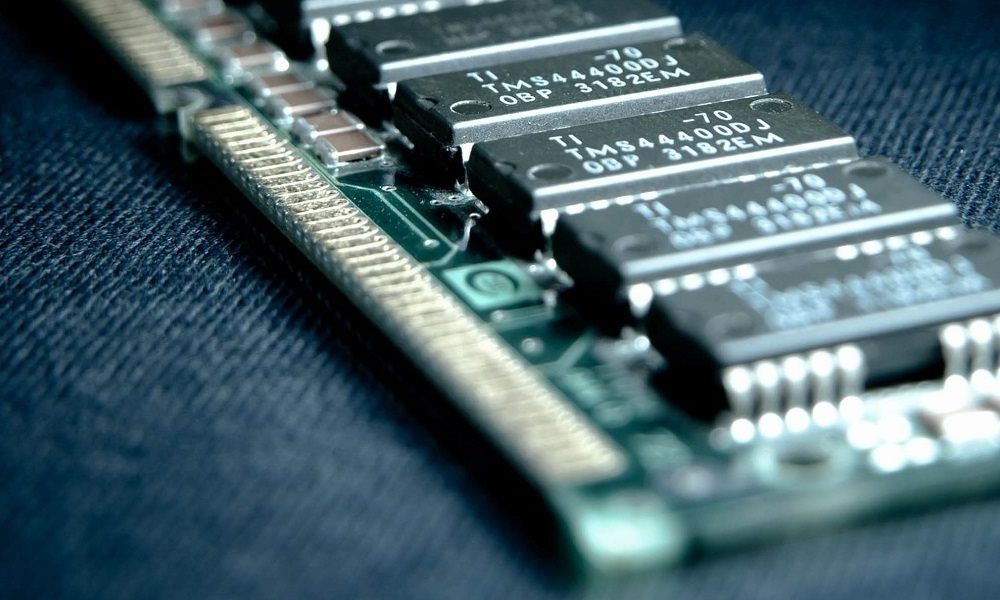
\includegraphics[width=4cm]{memoria-RAM.jpg}\centering
\caption{Memoria RAM}
\label{fig:memoria-RAM}
\end{figure}
\newline
\textbf{Memoria ROM:} Memoria de solo lectura.
\newline
\newline
"La memoria ROM es el medio de almacenamiento de programas o datos que permiten el buen funcionamiento de los ordenadores o dispositivos electrónicos a través de la lectura de la información sin que pueda ser destruida o reprogramable. El significado de memoria ROM es “Read Only Memory” traducido al español “Memoria de solo lectura.”
\newline
La memoria ROM es conocida como memoria no volátil ya que la información contenida en ella no es borrable al apagar el dispositivo electrónico.
\newline
La memoria ROM se encuentra instalada en la tarjeta madre “motherboard” lugar donde se encuentra la información básica del equipo, llamada “BIOS.”"\cite{ROM}
\newline
\newline
A continuación se presenta la imagen de una memoria ROM (\ref{fig:memoria-ROM})
\begin{figure}[h]
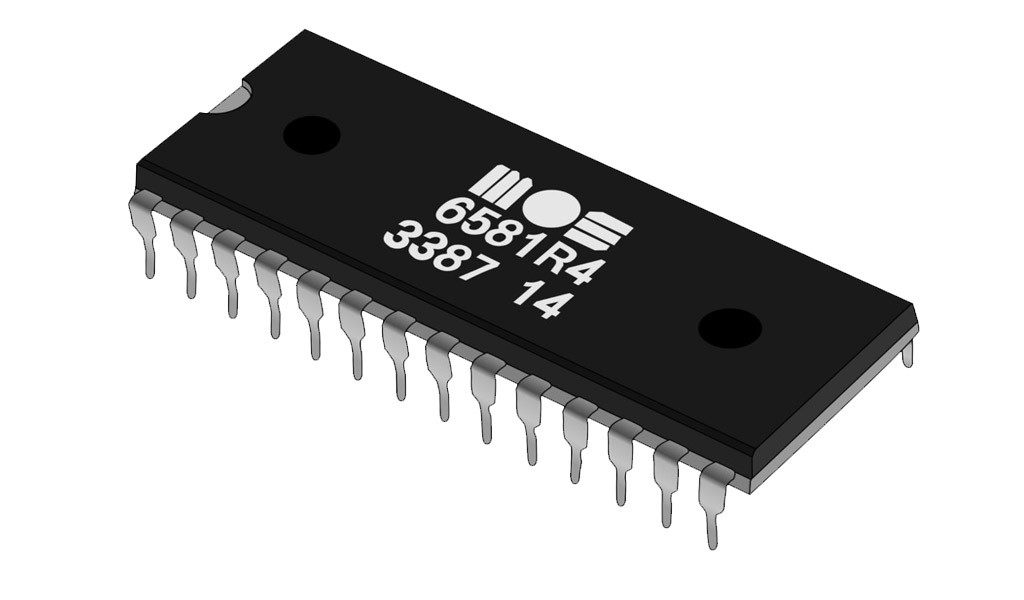
\includegraphics[width=4cm]{memoria-ROM.jpg}\centering
\caption{Memoria ROM}
\label{fig:memoria-ROM}
\end{figure}
\newline 
\newline 
\textbf{Memoria cache}
\newline
\newline
"Se conoce como memoria caché o memoria de acceso rápido a uno de los recursos con los que cuenta una CPU (Central Processing Unit, o sea, Unidad Central de Procesamiento) para almacenar temporalmente los datos recientemente procesados en un búfer especial, es decir, en una memoria auxiliar.
\newline
La memoria caché opera de modo similar a la Memoria Principal del CPU, pero con mayor velocidad a pesar de ser de mucho menor tamaño. Su eficacia provee al microprocesador de tiempo extra para acceder a los datos más frecuentemente utilizados, sin tener que rastrearlos a su lugar de origen cada vez que sean necesarios."\cite{Cache}
\newline
\newline
\textbf{Memoria RAM Dinámica (Dynamic DRAM)}
\newline
\subsection{¿Como se gestiona la memoria en el computador?}

A continuación se presenta el logo de C++ Figura (\ref{fig:cpplogo})

\begin{figure}[h]

\includegraphics[width=4cm]{cpplogo.png}
\centering
\caption{Logo de C++}
\label{fig:cpplogo}
\end{figure}

En la sección de teoremas (\ref{contenido})

\section{Conclusión} \label{conclulsion}

\bibliographystyle{IEEEtran}
\bibliography{references}

\end{document}
